\documentclass[lmodern, utf8, zavrsni]{fit}

%\batchmode
%\usepackage{booktabs}
\usepackage{listings}
\usepackage{longtable}
\usepackage{xcolor}
\usepackage{float}
\usepackage{enumitem}
\usepackage{hyperref}
\usepackage{enumerate}
\usepackage{graphicx}
\usepackage{etoolbox}
\usepackage{datetime}
\usepackage{needspace}
\usepackage{titlesec}
\usepackage{footnote}
%\titleformat{\chapter}[display]{\normalfont\huge\bfseries}{\chaptertitlename\ \thechapter}{20pt}{\Huge}

\begin{document}

\widowpenalty=300
\clubpenalty=300
\setlength{\parindent}{0pt}

\lstset{
  language=bash,
  backgroundcolor=\color{gray!25},
  basicstyle=\ttfamily \footnotesize,
  breaklines=true,
  prebreak=\raisebox{0ex}[0ex][0ex] {\ensuremath{\hookleftarrow}},
  columns=fullflexible,
  keywords={},
  mathescape=false
}


% this alters "before" spacing (the second length argument) to 0
%\titlespacing*{\chapter}{0pt}{0pt}{40pt}

% this changes "before" spacing back to its default of 50pt
%\titlespacing*{\chapter}{0pt}{50pt}{40pt}}

%\titlespacing*{\chapter}{0pt}{-50pt}{18pt}
%\titleformat{\chapter}[display]{\normalfont\huge\bfseries}{\chaptertitlename\ \thechapter}{20pt}{\Huge}

\title{Agilni \emph{software development}\newline \color{red}{(Nacrt)}}

\author{Ernad Husremović}
\brindex{DL 2792}
\verzija {0.1.0}
\thesisnumber{0000}
\mentor{doc. dr. Jasmin Azemović}

\maketitle

\tableofcontents

%\listoftables
%\listoffigures
\newpage

% abstract begin
%\begin{abstract}
%
%To be done 
%
%\keywords{open source software, OSS, Bosna i Hercegovina}
%\end{abstract}

% abstract end

\chapter{Uvod}
\vspace*{-0.7cm}

Šta znači `biti agilan'?

Agilni razvoj software-a ne predstavlja specifični proces. Agilni razvoj je način na koji se razmišlja o razvoju software-a\citep[str. 9]{agileart}.

Osnovna polazišta ovog pristupa opisuje "Agilni manifest"\footnote{\url{http://agilemanifesto.org/iso/en/principles.html}}, koji je definisan kroz četiri vrijednosti i 12 principa:

\section{Vrijednosti}

\begin{itemize}
\item Ljudi i interakcije ispred procesa i softverskih alata
\item \emph{Software} koji funkcioniše ispred detaljne dokumentacije
\item Komunikacija sa klijentima ispred pregovora
\item Odgovor na promjene ispred slijeđenja plana
\end{itemize}

\section{Principi}

\begin{itemize}
\item Glavni prioritet je zadovoljiti zahtjeve klijente kroz ranu i kontinuiranu \emph{isporuku} software-a
\item Blagonaklono prihvatiti \emph{promjene} funkcionalnih zahtjeva, čak i u kasnijim fazama razvoja.
\item Funkcionalan software treba isporučivati \emph{često}, nakon par hefti ili mjeseci, nastojeći da taj period bude što kraći.
\item Najefikasniji način razmejene informacija unutar razvojnog tima je direktna - `face-to-face' komunikacija.
\item Software koji \emph{funkcioniše} je primarna mjera uspjeha projekta.
\item Agilni procesi promoviraju održivi razvoj. Finansijeri, developeri i korisnici trebaju biti u stalnoj koordinaciji, bez obzira na dužinu trajanja projekta.
\item Kontinuirano pažnja na \emph{kvalitet} tehničkih operacije i dobar dizajn povećava agilnost.
\item \emph{Jednostavnost}, kao vještina postizanja maksimalnog učinka sa što manje rada, je krucijalni agilni princip.
\item Najbolja arhitektura, funkcionalni zahtjevi i dizajn se postižu u \emph{samo-organizovanim} timovima.
\item Tim redovno analizira predhodne operacije u cilju bolje efektivnosti (\emph{refleksija}). Na osnovu tih rezultata, tim utvrđuje buduće operacije.
\end{itemize}

Nijedan proces nije savršen. Svaki pristup razvoju software-a ima prostora za unapređenje. Konačno, cilj je ukloniti svaku barijeru između razvojnog tima i uspjeha projekta, pri čemu se pristup razvoju postupno adaptira novonastalim promjenama\emph{uslova}. To je agilnost.\citep[str 355]{agileart}

Agilni development koristi ''feedback'' u cilju konstantnih prilagodbi djelovanja, u visoko kolaborativnom okruženju. \citep{agileprag}

\section{Agilne metode}

Predmet detaljnijeg istraživanja su sljedeće agilne metode\footnote{\citep{agiledacs}}:
\begin{itemize}
  \item XP - \emph{Extreme programming}
  \item \emph{Scrum}
\end{itemize}

\begin{savenotes}
\begin{table}[ht]
\centering
\begin{tabular}{c c c c}
\hline\hline
Metoda & Dužina iteracije & Veličina tima & Distribucija tima\footnote{{Mogućnost da članovi tima budu geografski dislocirani, da ne sjede zajedno}} \\
\hline
   XP  & 1-2 hefte & 2-10 & Nije moguće \\
  Scrum & 2-4 hefte & 1-7 & Moguće \\ [1ex]
\hline
\end{tabular}
\label{table:methodkarakteristike}
\caption{Karakteristike pojedinih agilnih metoda}
\end{table}
\end{savenotes}

%\chater{Polazišne definicije \emph{Agilnog software development}-a}

\section{\emph{''Done Done''} princip}

Objasniti "done done" princip: Feature je done-done tek kada se može isporučiti klijentu.

\section{Tri nepobitne projektne istine}

Svaki projekat karakteriše sljedeće\citep{agilesamurai}
\begin{itemize}
  \item{Nemoguće je prikupiti sve zahtjeve klijenata na početku projekta}
  \item{Koliko god dobro prikupljni, zahtjevi klijenata će se mijenjati}
  \item{U svakom projektu će uvijek biti više posla nego li raspoloživih resursa (novca i vremena)}
\end{itemize}


\section{Organizacija i uloge unutar tima}

\subsection{XP organizacija tima}

\begin{itemize}
  \item{Product menadžer}
  \item{Couch}
  \item{Klijent}
  \item{Tester}
  \item{Developer}
\end{itemize}

\subsection{Scrum organizacija tima}

\begin{itemize}
    \item Product owner (PO)
    \item ScrumMaster
    \item The team
\end{itemize}

Note: Suštinske razlike u organizaciji između XP-a i Scrum-a ne postoje. 

\chapter{Početak projekta}

\section{Planiranje}

Generalno, agilni proces planiranja izbjegava detaljno ''head-on'' planiranje.

Objasniti šta znači "Addaptive planning"

\chapter{Analiza}

\section{\emph{Stories}}

Objasniti "Incremental requirements" princip.

Pragmatičan pristup analizi, analogno planiranju: analizira se do nivoa detalja koji se može postići u datom trenutku.

Definisanje detalja se vrši što je kasnije moguće, zato što tim kako projekat odmiče prikuplja sve više detalja - zato je razrada detalja kvalitetnija u kasnijim fazama projekta.

\subsection{\emph{Story card}}

Njihova glavna osobina je da su ''customer-centric'' - usmjereni na korisnika.  Svaka \emph{Story card} treba za cilj imati isporuku nove vrijednosti kljentu.

\section{Početne iteracije}

Početnim iteracijama se uspostavlja projekat, definiše toolset. U prvih par iteracija se takođe utvrđuje "velocity" tima.
U prvih par iteracija "velocity" značajno varira, dok se u kasnijim fazama "velocity" stabilizira.


\chapter{Praćenje projekta}
\vspace*{-0.7cm}

\subsection{Empirijska kontrola procesa}

Predefinisana kontrola procesa naspram empirijske kontrole procesa\citep{agiletransition}. Agilni pristup primjenjuje empirijsku kontrolu procesa.

\section{\emph{Trello} agilni projekt menadžment sistem}

\begin{figure}[H]
\centering
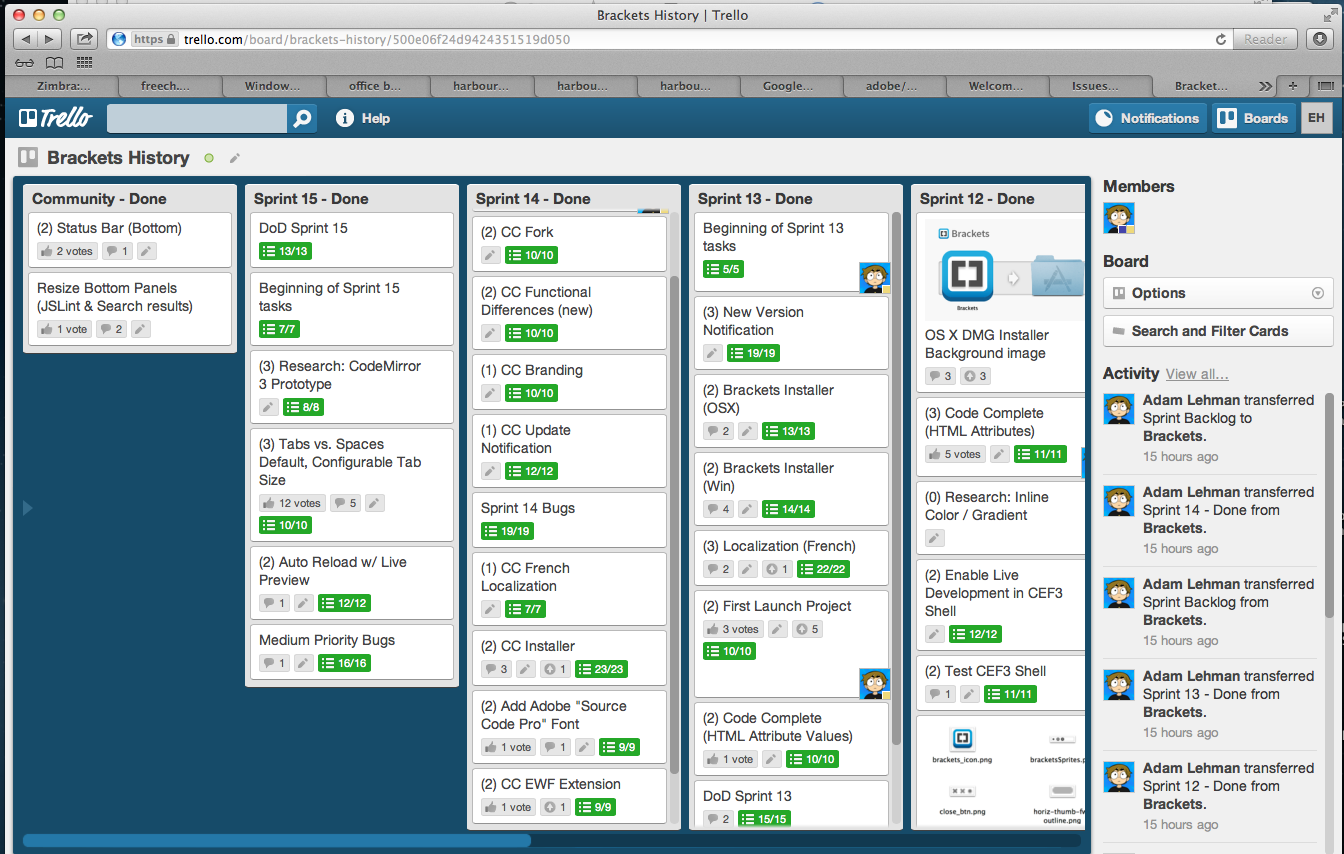
\includegraphics[width=10cm]{img/brackets_trello_sprint_history.png}
\caption{trello}
\end{figure}

\section{Slack}

Slack - "među-story" prostor\citep[str. 275]{agileart}

\section{Estimating}

Velocity, points,  Consistent Estimates

\subsection{Timeboxing, Iteration Timebox}

\section{Commitment}

Objasniti kada tim daje "commitment" u smislu realizacije plana.
Objasniti zašto je bitno da upravo tim vrši "estimating".

\chapter{Komunikacija}

\section{Review meetings}

Bez sastanaka nije moguće postići iterativnost. Stoga, je ovo obavezna praksa ASD-a.

\section{\emph{Issue management} (ISSUE)}

Zadatak, Aktivnost, ticket

''Issue''\footnote{developeri često koriste termin ''ticket'', ili ''bug'' (čak i kada se ne radi o programskog grešci)} predstavlja određeni kokretni projektni zadatak:
\begin{itemize}
  \item prijedlog za realizaciju (ideja)
  \item prijava programske greške (eng. bug)
  \item realizacija nove ili nadogradnja postojeće funkcije sistema (eng. new feature, feature upgrade)
\end{itemize}

\subsection{Poznati alati za \emph{issue management}}

\begin{itemize}
  \item gitlab issues\footnote{\citep{agilegit}}
  \item redmine issues\footnote{\url{http://www.redmine.org}, \url{http://redmine.bring.out.ba}}
\end{itemize}

Sve što je relevantno za projekat treba publikovati na ISSUE sitem.

Ako razvojni tim nije kolociran\footnote{Nalazi se i djeluje na jednom mjestu, nije geografski distribuiran} većina komunikacija između članova obavlja se elektronskim putem.

''Issues management'' sistem je po pitanju realizacije konkretnih projektnih zadataka najbolji način komunikacije.\footnote{email kao sredstvo komunikacije u ove svrhe treba izbjegavati. Email komunikacija brzo postaje nepregledna za većinu projektnih zadataka.}

Komunikacija putem ISSUE sistema time obuhvata komunikaciju na temu novih ideja i prijedloga, realizacije ili nadogradnje funkcija sistema, kao i prijavu i otklanjanje programskih ''bug''-ova (grešaka).

Parcijalni pristup (npr. ograničite se samo na ''bug''-ove) stvara prostor da bitne informacije budu nedostupne svim članovima tima.

Redovno nakon gornje preporuke slijedi pitanje:

Kako ću znati da li je nešto relevantno  ili nije ?

Ako ne znaš da li je relevantno - stavi na ''issue''. 

Nije nikakav problem da se na ticketima u početku nalaze suvišne informacije. Problem je kada informacije nedostaju.

Takođe je vrlo bitno da se informacije na sistem publikuju bez kašnjenje, a ne retroaktivno u formi izvještaja.

Mnoge informacije nakon dan ili dva postaju beskorisne.

Issue management treba reflektovanti život i dinamiku projekta.

\subsection{\emph{Issues} i novi član tima}

''Issues'' su sredstvo komunikacije.

Kada se novi član uključi u ekipu, redmine komentari (ili nedostatak komentara) su odličan indikator kompetencija člana.

Iz njih se vrlo brzo dođe do informacija kojim vještinama član raspolaže, koje su njegove profesionalne navike. Na osnovu tih informacija se može djelovati: 
\begin{itemize}
  \item Organizvati fokusiranu edukaciju za novog člana
  \item Zajednički rad sa iskusnijim kolegama itd.
\end{itemize}

\chapter{Agilni pristup dizajnu}

\section{Inkrementalni dizajn}

Izbjegava se zasebna, dugotrajna faza dizajna (''up-front''). 

To znači da se k\^odiranju (implementaciji) pristupa bez jasnog dizajna ?!

Zagovarači agilnih metoda developmenta na ovakva pitanja daju sljedeći odgovor:

\begin{quote}
   \emph{\large Smatrate da je dizajn zanemaren u agilnom software developmentu ? Upravo suprotno - Mi dizajn smatramo iznimno bitnim. Zato ga \textbf{prakticiramo} kroz \textbf{sve faze} razvojnog procesa !} 
\end{quote}


Suštinska razlika u odnosu na klasični ''up-front'' je ta da se dizajniranje realizira u onoj mjeri i u onom trenutku kada je to najpogodnije i najprirodnije za razvojni tim.

Prakticiranje inkrementalnog i jednostavnog dizajn zato spriječava ''overengineering''\footnote{http://en.wikipedia.org/wiki/Overengineering}

\section{Jednostavni dizajn}

\subsection{\emph{You Aren't Gonna Need It} (YAGNI)}

YAGNI\footnote{Ovo vam neće trebati} princip je bazni aspekt jednostavnog dizajna\footnote{\citep[str. 318]{agileart}}


\chapter{Development}

\section{\emph{Source code management} (SCM)}

Detaljno u materijalu ''Agilni \emph{software development}, GIT SCM''\citep{agilegit}

\section{Testiranje}

Testiranje i refactoring etaljno u materijalu ''Agilni \emph{software development}, Tehnike testiranja''\citep{agiletest}

Objasniti zašto je TDD ujedno i testiranje i implementacija(kodiranje) i dizajn !

\section{Stalna integracija (CI)}

Detaljno u materijalu ''Agilni \emph{software development}, \emph{Continuous Integration} (CI)''\citep{agileci}

\section{\emph{''Jednom i samo jednom''}}

''Jednom i samo jednom'' (eng. ''Once and Only once'') princip:

\begin{quotation}
  Svaki koncept izrazi jednom. (i samo jednom !).\footnote{\citep[str. 319]{agileart}}
\end{quotation}

\section{\emph{Spike} rješenja}

Spike (\href{http://translate.google.com/#en/hr/spike}{\color{blue}{bos. ekser, smeč}}) razjašnjavaju tehička pitanja koje susrećemo, pri čemu se izbjegava kompleksnost produkcijskog k\^oda.\citep[str. 334]{agileart}

\chapter{Release management}

\section{Testno vs produkcijsko okruženje}

Detaljno u materijalu ''Agilni \emph{software development}, \emph{Test} \& \emph{deploy} infrastruktura''\citep{agiletestdeploy}

\chapter{Ostalo}

\section{ASD vodi ka haosu ?!}

Striktne granice između faza dizajna, implementacije i isporuke rješenja korisniku nestaju.

Prakticiranjem TDD-a developer stalno mijenja dizajn\footnote{inkrementalni dizajn TODO: referenciraj se na poglavlje} u malim koracima u toku implementacije.

Breakthrough faze obezbjeđuju veće promjene. Bitno je uočiti da se te promjene dešavaju u najbolje, najproduktivnije vrijeme - onda kada developer ''sazrije'' po pitanju konkretnog problema, kada dobro ovlada postojećim stanjem - njegovim ograničenjima i dobrim stranama.

Što ne trebaš (čega nema u \emph{story}-jima) - ne implementiraj !

Nemamo potrebu anticiparti dizajnerska i arhitektonska rješenja na duge staze.

Nedostatak anticipacije će voditi ''siromašnim'', ''kratkovidnim'' rješenjima ?

ASD svakako nije pogodan za svaki tim. ASD doista može uzrokovati paralizu tima koji nije pripremljen za ASD.

\section{Rizici i ograničenja ASD-a}

Agilni \emph{software development} pretpostavlja visoko motiviran tim, tim koji je spreman da uči. 

Članovi tima moraju posjedovati bazne vještina iz oblasti koje pokrivaju.

Ako se te vještine i uvriježene prakse u slučaju programera svode na očekivanja prema vodećim članovima tima na:

\begin{quotation}
  \emph{Dajte vi meni šta trebam uraditi (izk\^odirati), to je sve što me interesuje (dalje od toga nije moj posao) !}
\end{quotation}

onda ovaj tim (još) \emph{nije spreman} za agilni development.

Agilni pristup jednostavno nudi i očekuje od svakog pojedinca da maksimalno doprinosi projektu u cjelini. Kolokvijalnim riječnikom, neprihvatljivo je da članovi tima probleme koji nisu direktno vezani za njihovu trenutnu aktivnost i zaduženja adresiraju kao:

\begin{quotation}
  \emph{To nije moj ''rejon'' !\footnote{Legendarna šala iz serije ''Nadrealisti''} ?}
\end{quotation}

Naravno da je i u agilnom timu neophodno poslove raporediti na najbolji način, te da je svaštarenje potrebno smanjiti na namanju moguću mjeru.
Međutim, treba uvijek imati na umu da je agilni tim multi-funkcionalan, usmjeren na ciljeve projekta.

Stoga je sve što ima bitan uticaj na ciljeve i tok projekta ''rejon'' svakog člana.

\section{Komptencije i vještine}

Potreban (ali ne i dovoljan) uslov u primjeni agilnih metoda su odgovarajuće kompetencije i veštine članova tima. Ako one ne postoje, agilni pristup će doživjeti potpuni fjasko.

Ovdje treba naglasiti da se prvenstveno misli na bazne kompetencije i vještine, ne kompentencije koje se stiču dugogodišnjim iskustvom. Naravno, iskusniji članovi, članovi koji posjeduju višegodišnjim iskustvom iz problemskog domena projekta su bitan faktor.\footnote{Ako projekat ima kratke rokove za realizaciju, najčešće i neophodan} Međutim, tim koji je spreman da uči može nadoknaditi nedostatak iskustva. Takav tim zasigurno neće moći brzo realizovati ciljeve projekta, ali će pravilnim pristupom doći do cilja.

\subsection{Eksperti i izvršioci}

U nedostatku kompetencija se pribjegava klasičnom hijerarhijskom sistemu\footnote{''vojni'' sistem} u kome unutar tima postoje jedan - dva eksperta\footnote{ekspert = ''guru''}, dok ostatak tima (i većinski dio tima) čine krajnji izvršioci\footnote{izvršioc = ''hamal''}

Note: Ovdje je bitno razgraničiti da se od junior programera ili novog člana tima naravno ne može očekivati previše, ali je ključna stvar postići visoku dinamičnost njegove pozicije od početnika do člana koji daje značajan doprinos projektu.


\section{Agilni software development u \emph{Opensource} projektima}

Most of the analyzed projects adapted a fixed cycle and others are in the process of transition. Fixed cycles can also be found in agile software engineering methods, such as Extreme Programming or the Scrum method. While not equal to those methods, the analyzed projects seem to benefit from such an approach. The release schedule with fixed cycles is often already fixated before development starts and each project tries to stick to it as close as possible.\citep[str. 95]{Siegel2012}

As shown by Mockus, Fielding and Herbsleb the role of the release manager is vital for every project.\citep[str. 95]{Siegel2012}

\chapter{Zaključak}

Agilni \emph{software development} svakako nije \emph{Silver Bullet}\footnote{\url{http://en.wikipedia.org/wiki/No_Silver_Bullet}}

Međutim, on iz temelja mijenja uvriježene inžinjerske prakse. Agilni pristup unosi ''životnost'' u razvojni proces software-a.

U toku razvoja sofware-a\footnote{ali i sveukupnog životnog ciklusa} se od članova razvojnog tima u znak rezignacije mogu čuti konstatacije slijedećeg tipa:
\begin{quotation}
  \emph{Hah, sve bi bilo u redu da živimo u idealnom svijetu ... Da imamo dovoljno vremena i/ili developera ... Da smo prije implementacije ''xyz'' funkcije dobili sve potrebne informacije ...}
\end{quotation}

Agilni pristup kao temeljno polazište uzima realni svijet i realne potrebe korisnika software-a.

On razvojni tim stalno podsjeća i usmjerava da je glavni cilj sofverskog projekta ostvariti vrijednost za \emph{korisnika software}-a.\footnote{Prvi slogan moje firme je bio: \emph{Iskoristite računar}. Međutim, slogan se nije puno koristio. Još gore, firma u svom djelovanju u mnogim segmentima odstupila od principa ovog slogana. Nakon 16 godina, rad na ovoj temi me je podsjetio na taj slogan. Iz ove perspetkive mogu konstatovati da je to bio sjajan slogan. Šteta što smo ga zaboravili - i slovom i djelom.}
Ta vrijednost (upotrebljivost, korisnost) je sama po sebi vremenski \emph{dinamična} kategorija. Agilni \emph{software development} nastoji razvojni ciklus usaglasiti sa tom činjenicom.

Agilni pristup zahtjeva visok nivo kompetencija unutar tima, te postojanje kulture učeće organizacije\footnote{\url{http://en.wikipedia.org/wiki/Learning_organization}}.


% -------------------------------------------------
\bibliography{literatura}
\bibliographystyle{fit}

% -------------------------------------------------
\appendix

\chapter{Riječnik termina}

\begin{itemize}
  \item Coach - mentor razvojnog tima, onaj koji se brine o primjeni praksi, moderira tok procesa i komunikaciju unutar tima
  \item Velocity - sposobnost, kapacitet tima u toku iteracije
\end{itemize}



\chapter{Software toolset}
\begin{enumerate}
  \item Mac OS X 10.8.2
  \item mvim, vim tekst editor ver 7.3
  \item MacTex (TeX Live 2012)
\end{enumerate}

\chapter{Software repozitoriji}

\begin{itemize}
  \item Agilni developerski environment - \url{https://github.com/hernad/agile\_dev\_env}

\end{itemize}

\end{document}
